%%
%% kit-prog-tutorial
%%
%% Slides for my Java programming tutorial at KIT using LaTeX beamer.
%%
%% Copyright (c) 2015-2016 YouniS Bensalah <younis.bensalah@gmail.com>
%%
%% This work is released to the public domain.
%% For the full copyright and license information, please view the LICENSE file.
%%

\documentclass[18pt]{beamer}

\usepackage{templates/beamerthemekit}

\usepackage[utf8]{inputenc}
\usepackage{hyperref}
\usepackage{listings}
\usepackage{xcolor}
\usepackage{colortbl}

\titleimage{road}

\definecolor{lime}{HTML}{8FFF53}

\newcommand{\tagline}{Lists and Abstract Data Types}

\newcommand{\quotes}[1]{``#1''}

\title[Programmieren\hspace{2.5pt}--\hspace{2.5pt}\tagline]{\tagline}
\subtitle{Programmieren~\textbar~Tutorium 32}

\author{YouniS Bensalah}
\date{5. Dezember 2016}

\institute{Chair for Software Design and Quality}

\usepackage[citestyle=authoryear,bibstyle=numeric,hyperref,backend=biber]{biblatex}
\addbibresource{templates/example.bib}
\bibhang1em

\begin{document}

% remove annoying figure prefix in caption
\setbeamertemplate{caption}{\raggedright\insertcaption\par}

\selectlanguage{english}

\begin{frame}
    \titlepage
\end{frame}

% \begin{frame}{Heute}
%     \tableofcontents
% \end{frame}

\section{Listen und abstrakte Datentypen}

\begin{frame}{Listen und abstrakte Datentypen}
    \begin{figure}
        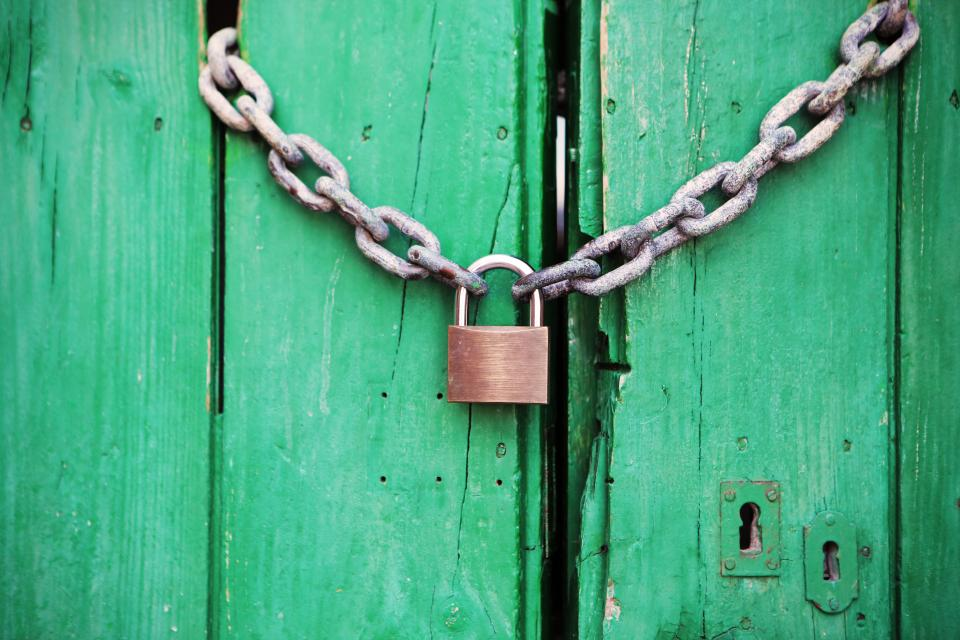
\includegraphics[scale=.3]{img/AD76394B17.jpg}
    \end{figure}
\end{frame}

\begin{frame}{Rekursive Datentypen}
    \begin{block}{}
        Ein Datentyp ist \textit{rekursiv}, wenn Objekte Verweise auf Objekte derselben Klasse enthalten.
    \end{block}
\end{frame}


\subsection{Verkettete Listen}

\begin{frame}{Verkettete Listen}
    \begin{block}{}
        Eine \textbf{verkettete Liste} ist eine dynamische Datenstruktur, bei der jedes Element auf seinen Nachbarn verweist.
    \end{block}

\end{frame}

\begin{frame}{Verkettete Listen}
    Verkettete Listen sind ein \textit{rekursiver Datentyp}.
\end{frame}

\begin{frame}{Einfach verkettete Listen}

    \begin{itemize}
        \item Bei einer \textbf{einfach verketteten Liste} zeigt jedes Element auf das nächste Element in der Liste
        \item Jedes Element enthält auch den eigentlichen Inhalt der Zelle
        \item Das letzte Element zeigt auf \texttt{null}
    \end{itemize}

    \begin{figure}
        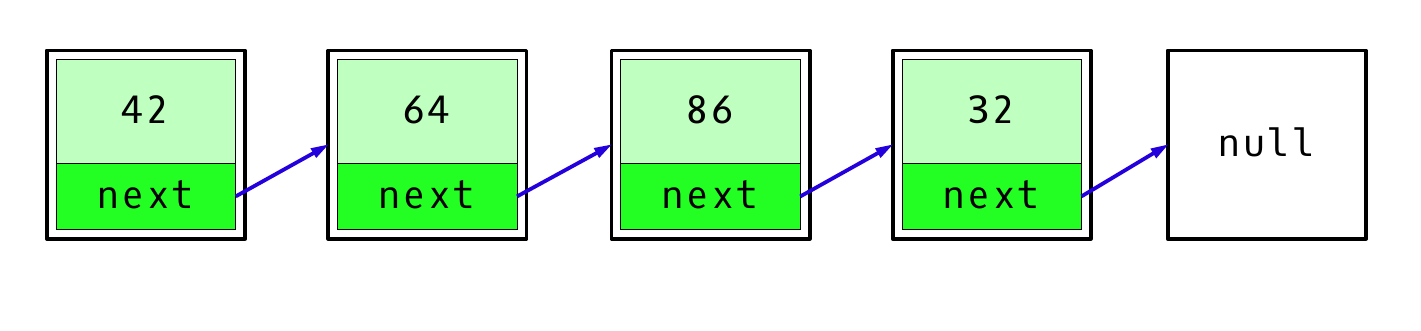
\includegraphics[scale=.3]{img/simplelinkedlist.png}
    \end{figure}

\end{frame}

\begin{frame}[fragile]{Einfach verkettete Listen}

    Implementierung in Java\dots

    \begin{exampleblock}{}
        \begin{lstlisting}[language=Java]
public class Cell {
    private int content;
    private Cell next;
}
        \end{lstlisting}
    \end{exampleblock}

\end{frame}

\begin{frame}[fragile]{Einfach verkettete Listen}

    \begin{exampleblock}{}
        \begin{lstlisting}[language=Java,basicstyle=\scriptsize]
public class Cell {
    private int content;
    private Cell next;

    public Cell(int content, Cell next) {
        this.content = content;
        this.next = next;
    }

    public Cell getNext() { return this.next; }
    public void setNext(Cell next) { this.next = next; }
    public int getContent() { return this.content; }
    public void setContent(int content) { this.content = content; }
}
        \end{lstlisting}
    \end{exampleblock}

\end{frame}


\begin{frame}[fragile]{Einfach verkettete Listen}

    \begin{exampleblock}{}
        \begin{lstlisting}[language=Java,basicstyle=\scriptsize]
Cell c3 = new Cell(32, null);    // c3 --> null
Cell c2 = new Cell(99, c3);      // c2 --> c3
Cell c1 = new Cell(42, c2);      // c1 --> c2
        \end{lstlisting}
    \end{exampleblock}

\vspace{.2in}

\pause

Das erste Element (\texttt{head}) genügt, um komplette Liste zu durchlaufen!

\end{frame}


\begin{frame}{Operationen auf verketteten Listen}
    \begin{itemize}
        \item \textbf{Einfügen} von Listenelementen\\
        \texttt{addFirst}, \texttt{addLast}
        \item \textbf{Löschen} von Listenelementen\\
        \texttt{remove}
        \item \textbf{Suchen} nach Listenelementen\\
        \texttt{contains}
        \item \dots
    \end{itemize}
\end{frame}

\begin{frame}[fragile]{Operationen auf verketteten Listen}
    Wir fassen nun die aneinanderhängenden Listenelemente zu einer Klasse \textbf{Liste} zusammen.

    \begin{exampleblock}{}
        \begin{lstlisting}[language=Java,basicstyle=\scriptsize]
public class List {
    private Cell head;

    public List(Cell head) {
        this.head = head;
    }
}
        \end{lstlisting}

    \end{exampleblock}


\end{frame}

\begin{frame}{Einfügen}
    \textbf{Einfügen} von Listenelementen an Anfang oder Ende der Liste
\end{frame}


\begin{frame}[fragile]{Einfügen}
    \begin{exampleblock}{addFirst}
        \begin{lstlisting}[language=Java,basicstyle=\scriptsize]
public void addFirst(int content) {
    Cell c = new Cell(content, this.head);
    this.head = c;
}
        \end{lstlisting}

    \end{exampleblock}

\end{frame}

\begin{frame}[fragile]{Einfügen}

    \begin{exampleblock}{addLast}
        \begin{lstlisting}[language=Java,basicstyle=\scriptsize]
public void addLast(int content) {
    if (this.head == null) {
        this.head = new Cell(content, null);
        return;
    }

    Cell c = this.head;
    while (c.getNext() != null) {
        c = c.getNext();
    }
    c.setNext(new Cell(content, null));
}
        \end{lstlisting}

    \end{exampleblock}

\end{frame}

\begin{frame}{Löschen}
    \textbf{Löschen} von Listenelementen
\end{frame}

\begin{frame}[fragile]{Löschen}
    \begin{exampleblock}{remove}
        \begin{lstlisting}[language=Java,basicstyle=\scriptsize]
public void remove(int content) {
    Cell c = this.head;

    while (c != null && c.getContent() == content) {
        this.head = c.getNext();
        c = this.head;
    }

    if (c == null) {
        return;
    }

    while (c.getNext() != null) {
        if (c.getNext().getContent() == content) {
            c.setNext(c.getNext().getNext());
        } else {
            c = c.getNext();
        }
    }
}
        \end{lstlisting}

    \end{exampleblock}

\end{frame}

\begin{frame}{Suchen}
    \textbf{Suchen} nach Listenelementen
\end{frame}

\begin{frame}[fragile]{Suchen}
    \begin{exampleblock}{contains}
        \begin{lstlisting}[language=Java,basicstyle=\scriptsize]
public boolean contains(int content) {
    for (Cell c = this.head; c != null; c = c.getNext()) {
        if (c.getContent() == content) {
            return true;
        }
    }
    return false;
}
        \end{lstlisting}

    \end{exampleblock}

\end{frame}


\begin{frame}{Doppelt Verkettete Listen}
    \begin{itemize}
        \item Jedes \textbf{Listenelement} merkt sich sowohl das \textbf{nächste} (\texttt{next}) als auch das \textbf{vorherige} (\texttt{prev}) Element
        \item \textbf{Liste} merkt sich dann sowohl \textbf{Anfang} (\texttt{head}) als auch \textbf{Ende} (\texttt{tail}) der Liste
        \item Liste kann \textit{vorwärts} wie \textit{rückwärts} traversiert werden
        \item \texttt{addLast}-Operation jetzt in $\mathcal{O}(1)$ möglich!
    \end{itemize}

    \begin{figure}
        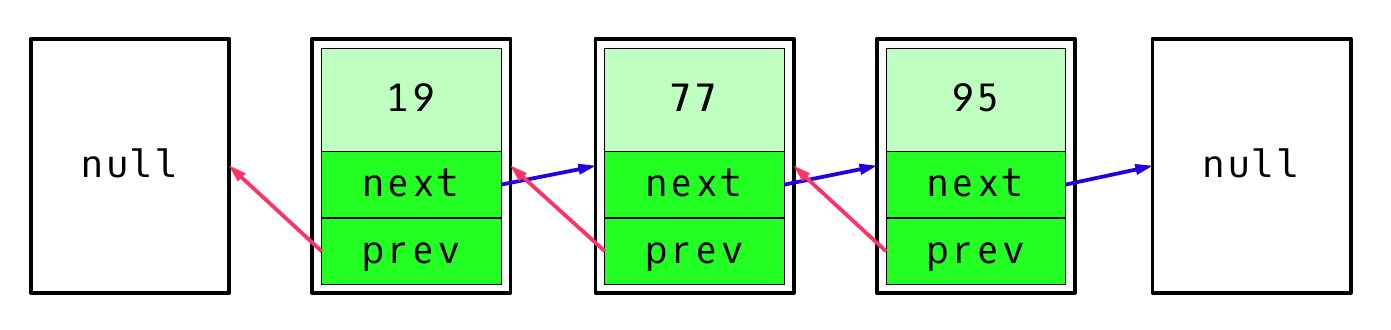
\includegraphics[scale=.3]{img/doublelinkedlist.png}
    \end{figure}
\end{frame}

\begin{frame}{Listen vs. Arrays}
    \begin{itemize}
        \item \textbf{Listen}
        \begin{itemize}
            \item Dynamische Größe
            \item Einfaches Einfügen und Löschen von Elementen
            \item Zugriff auf innere Elemente nur durch Traversierung der Liste möglich
        \end{itemize}
        \item \textbf{Arrays}
        \begin{itemize}
            \item Statische Größe
            \item Einfacher Zugriff auf beliebige Elemente in $\mathcal{O}(1)$
            \item Cache-effizient
        \end{itemize}
    \end{itemize}
\end{frame}


\subsection{Abstrakte Datentypen}

\begin{frame}{Abstrakte Datentypen}
    \begin{block}{}
        Ein \textbf{abstrakter Datentyp} beschreibt eine Menge von Typen in Kombination mit zulässigen Operationen.
    \end{block}

\end{frame}

\begin{frame}{Abstrakte Datentypen: Geheimnisprinzip}
    \begin{itemize}
        \item \textbf{Abstrakte Sicht auf die Liste}
        \item Wenn wir eine Liste nur als solche verwenden wollen, interessiert uns der interne Aufbau nicht
    \end{itemize}

\end{frame}


\begin{frame}{Abstrakte Datentypen: Datenkapselung}
    \begin{alertblock}{}
        \begin{itemize}
            \item Ein abstrakter Datentyp trifft \textit{keine} Aussagen über konkrete Implementierung
            \item Prinzip der Datenkapselung
            \item Zugriff auf Inhalt der Liste nur über definierte Schnittstelle
        \end{itemize}
    \end{alertblock}

\end{frame}

\subsection{Iterator}


\begin{frame}{Iterator}
    \begin{block}{}
        Ein \textbf{Iterator} ist ein Zeiger, mit dem die Elemente einer Datenstruktur\\ (z. B. Liste) durchlaufen werden können.
    \end{block}

\end{frame}

\begin{frame}[fragile]{Iterator}

    \begin{exampleblock}{}
        \begin{lstlisting}[language=Java,basicstyle=\scriptsize]
public class List {
    // ...
    public class Iterator {
        private Cell cursor;
        private Iterator(Cell start) { this.cursor = start; }
        public boolean hasNext() { return this.cursor != null; }
        public int next() {
            int c = this.cursor.getContent();
            this.cursor = this.cursor.getNext();
            return c;
        }
    }

    public Iterator iterator() {
        return new Iterator(this.head);
    }
}
        \end{lstlisting}

    \end{exampleblock}

\end{frame}

\begin{frame}[fragile]{Iterator}

    \begin{exampleblock}{}
        \begin{lstlisting}[language=Java]
List myList;
// ...

List.Iterator it = myList.iterator();
while (it.hasNext()) {
    int x = it.next();
    doWork(x);
}
        \end{lstlisting}

    \end{exampleblock}

\end{frame}

\appendix
\beginbackup

\section{Graphen}

\subsection{Knoten und Kanten}

\begin{frame}{Graphen}
    \begin{figure}
        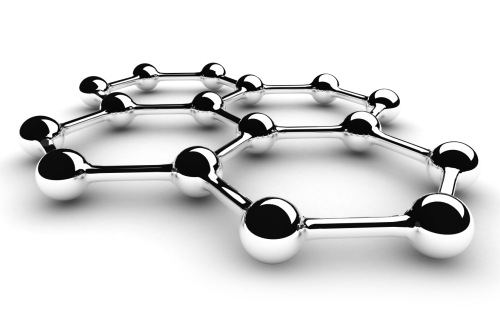
\includegraphics[scale=2.5]{img/graph.jpg}
    \end{figure}
\end{frame}

\begin{frame}{Graphen}
    \begin{block}{Definition}
        Ein \textbf{Graph} ist ein Paar $\mathcal{G} = (\mathcal{V}, \mathcal{E})$
        mit $\mathcal{V}$ Menge von Knoten
        und $\mathcal{E} \subset \mathcal{V} \times \mathcal{V}$ Menge von Kanten.
    \end{block}

\end{frame}


\begin{frame}{Graphen}
        \begin{figure}
            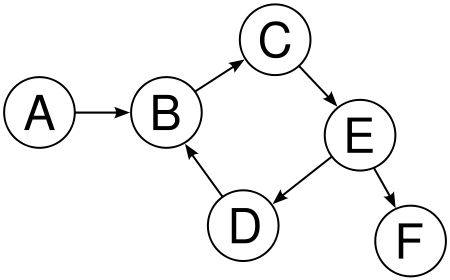
\includegraphics[scale=.5]{img/graph.png}
        \end{figure}

\end{frame}


\begin{frame}{Graphen}

        \begin{exampleblock}{}
            \begin{itemize}
                \item $\mathcal{V} = $ ?
                \item $\mathcal{E} = $ ?
            \end{itemize}
        \end{exampleblock}


        \begin{figure}
            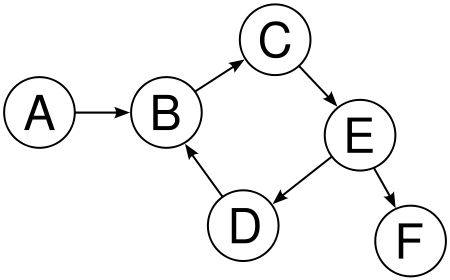
\includegraphics[scale=.3]{img/graph.png}
        \end{figure}

\end{frame}

\begin{frame}{Graphen}

        \begin{exampleblock}{}
            \begin{itemize}
                \item $\mathcal{V} = \left\{ A, B, C, D, E, F \right\}$
                \item $\mathcal{E} = \left\{ (A, B), (B, C), (C, E), (D, B), (E, D), (E, F) \right\}$
            \end{itemize}
        \end{exampleblock}


        \begin{figure}
            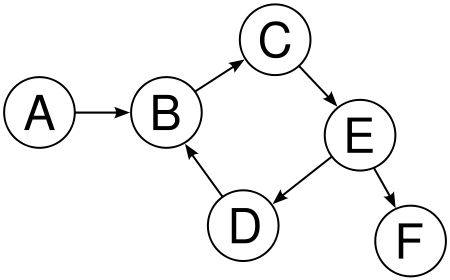
\includegraphics[scale=.3]{img/graph.png}
        \end{figure}

\end{frame}

\begin{frame}{Darstellung von Graphen}
    \textbf{Problem:} Wie kann ich einen Graphen in meinem Programm darstellen?
\end{frame}


\subsection{Adjazenzmatrix}

\begin{frame}{Adjazenzmatrix}
    \[
    \left(
    \begin{array}{cccccc}
        0 & 1 & 0 & 0 & 0 & 0 \\
        0 & 0 & 1 & 0 & 0 & 0 \\
        0 & 0 & 0 & 0 & 1 & 0 \\
        0 & 1 & 0 & 0 & 0 & 0 \\
        0 & 0 & 0 & 1 & 0 & 1 \\
        0 & 0 & 0 & 0 & 0 & 0
    \end{array}
    \right)
    \]

    \begin{figure}
        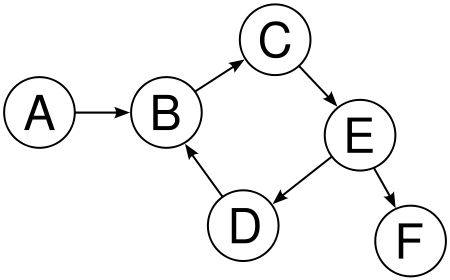
\includegraphics[scale=.3]{img/graph.png}
    \end{figure}

\end{frame}


\begin{frame}{Adjazenzmatrix}
    \[
    \left(
    \begin{array}{cccccc}
        0 & 1 & 0 & 0 & 0 & 0 \\
        0 & 0 & 1 & 0 & 0 & 0 \\
        0 & 0 & 0 & 0 & 1 & 0 \\
        0 & 1 & 0 & 0 & 0 & 0 \\
        0 & 0 & 0 & 1 & 0 & 1 \\
        0 & 0 & 0 & 0 & 0 & 0
    \end{array}
    \right)
    \]

    \begin{itemize}
        \item Adjazenzmatrix speichert, welche Knoten des Graphen durch eine Kante verbunden sind
        \item Zeilen entsprechen den Startknoten, Spalten entsprechen den Zielknoten
        \item $1$ bedeutet, dass eine Kante existiert, $0$ bedeutet, dass die Knoten \textit{nicht} verbunden sind
    \end{itemize}

\end{frame}

\begin{frame}[fragile]{String.split}
    \begin{lstlisting}[language=Java]
String[] split(String regex)
    \end{lstlisting}


    \begin{itemize}
        \item \texttt{String.split} zerlegt eine Zeichenkette nach einem gegebenen Muster
        \item Als Rückgabe erhält man einen Array mit den einzelnen Stücken
    \end{itemize}

\begin{exampleblock}{}
    \begin{lstlisting}[language=Java,basicstyle=\scriptsize]
String colors = "cyan;yellow;magenta";
String[] result = colors.split(";");
    \end{lstlisting}
\end{exampleblock}

\begin{itemize}
    \item Der Array \texttt{result} enthält jetzt\\ \texttt{\{ "cyan", "yellow", "magenta" \}}
\end{itemize}

\end{frame}

\begin{frame}{Gleichheit von Objekten}
    \begin{itemize}
        \item In Java gibt es zwei Möglichkeiten, auf Gleichheit zu prüfen
        \begin{itemize}
            \item \texttt{"=="}\\
            Prüft auf Wert-Gleichheit

            \item \texttt{equals}\\
            Prüft auf inhaltliche Objekt-Gleichheit
        \end{itemize}
        \item Klasse kann \texttt{equals}-Methode \textbf{überladen} und Gleichheit von zwei Objekten selbst definieren
        \item \alert{Bei \textbf{Objekten} ist Wert-Gleichheit gerade \textbf{Gleichheit der Referenz}!}
    \end{itemize}
\end{frame}

\begin{frame}{Fragen?}
    \begin{figure}
        
\includegraphics[scale=.32]{img/Question-Rage-Face.jpg}
    \end{figure}
\end{frame}

\begin{frame}{Bis nächste Woche!}
    \begin{figure}
        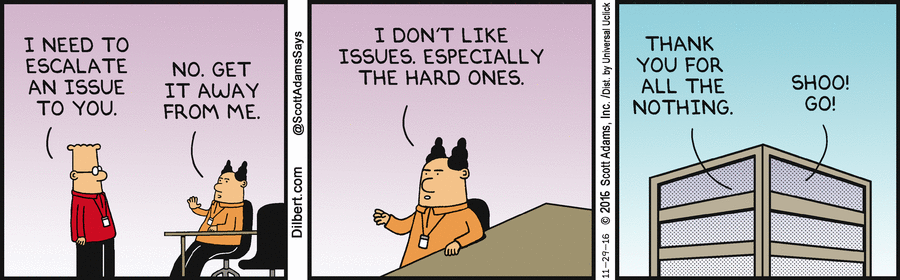
\includegraphics[scale=.5]{img/dt161129.png}
        \caption{\footnotesize{dilbert.com}}
    \end{figure}
\end{frame}

\backupend

\end{document}
